% Latex2e homework template for 14-741/18-631 taught by Nicolas Christin
%
\documentclass[12pt]{article}  % Decrease to 10pt if desired

\usepackage[letterpaper,margin=1in]{geometry}
\usepackage{times}
\usepackage{ragged2e}
\usepackage{lastpage}
\usepackage{fancyhdr}
\usepackage{url}
\usepackage{mathtools}
\usepackage{listings}
\usepackage{graphicx}
\usepackage[font=small,skip=0pt]{caption}
\usepackage{tabu}
\pagestyle{fancy}
\addtolength{\parskip}{\baselineskip} %--skip lines between paragraphs
\setlength{\parindent}{0pt} %--don't indent paragraphs
\AtBeginDocument{\raggedright}

%
% Set your personal information here
%
\newcommand{\FirstName}{Shi}
\newcommand{\LastName}{Su}
\newcommand{\AndrewID}{shis}
\newcommand{\CourseNumber}{14-741}
\newcommand{\Campus}{PIT}  % Either PIT or Kobe

%
% Set assignment date here
%
\newcommand{\Date}{11/20/2015}


% Set up headers
\renewcommand{\headrulewidth}{0pt}
\setlength{\headheight}{0.5in}
\lhead{\FirstName~\LastName\\\AndrewID}
\chead{}
\rhead{\CourseNumber~/~\Campus\\\Date}
\lfoot{}
\cfoot{}
\rfoot{Page \thepage~of \pageref{LastPage}}

%Answer block
\newenvironment{answer}{
\setlength\parindent{24pt}
%\par\addvspace{\baselineskip}
}


%
% Begin document
%
\begin{document}

%
% Problem 1
%
\begin{center}
\textbf{Problem \#1 : Using Tor}
\end{center}
\parskip 0pt

%
% Problem 1: Preliminaries
%
 \subsubsection*{1.1 Preliminaries}
1. What is your public IP address?\\
\begin{answer}
Public IP address: {\bf 128.237.200.1}\\
Result of whois:
%\hspace{10em}
\begin{lstlisting}[basicstyle=\linespread{0.5}]
NetRange:       128.237.0.0 - 128.237.255.255
CIDR:           128.237.0.0/16
NetName:        CMU-NET-128-237
NetHandle:      NET-128-237-0-0-1
Parent:         NET128 (NET-128-0-0-0-0)
NetType:        Direct Assignment
OriginAS:       AS9
Organization:   Carnegie Mellon University (CARNEG-Z)
RegDate:        1987-05-06
Updated:        2012-04-02
Ref:            http://whois.arin.net/rest/net/NET-128-237-0-0-1
\end{lstlisting}
Complete output available in {\bf shis\_hw4\slash whois.txt}
\end{answer}
\bigskip

2. Display all Tor circuits your machine currently uses, as specified by the list of three Tor relays.\\
\begin{answer}
Script available in {\bf shis\_hw4\slash circuits.py}\\
It assumes that {\bf tor} is installed and already launched tor with {\bf ControlPort: 9151}\\
\begin{figure}[h]
\centering
  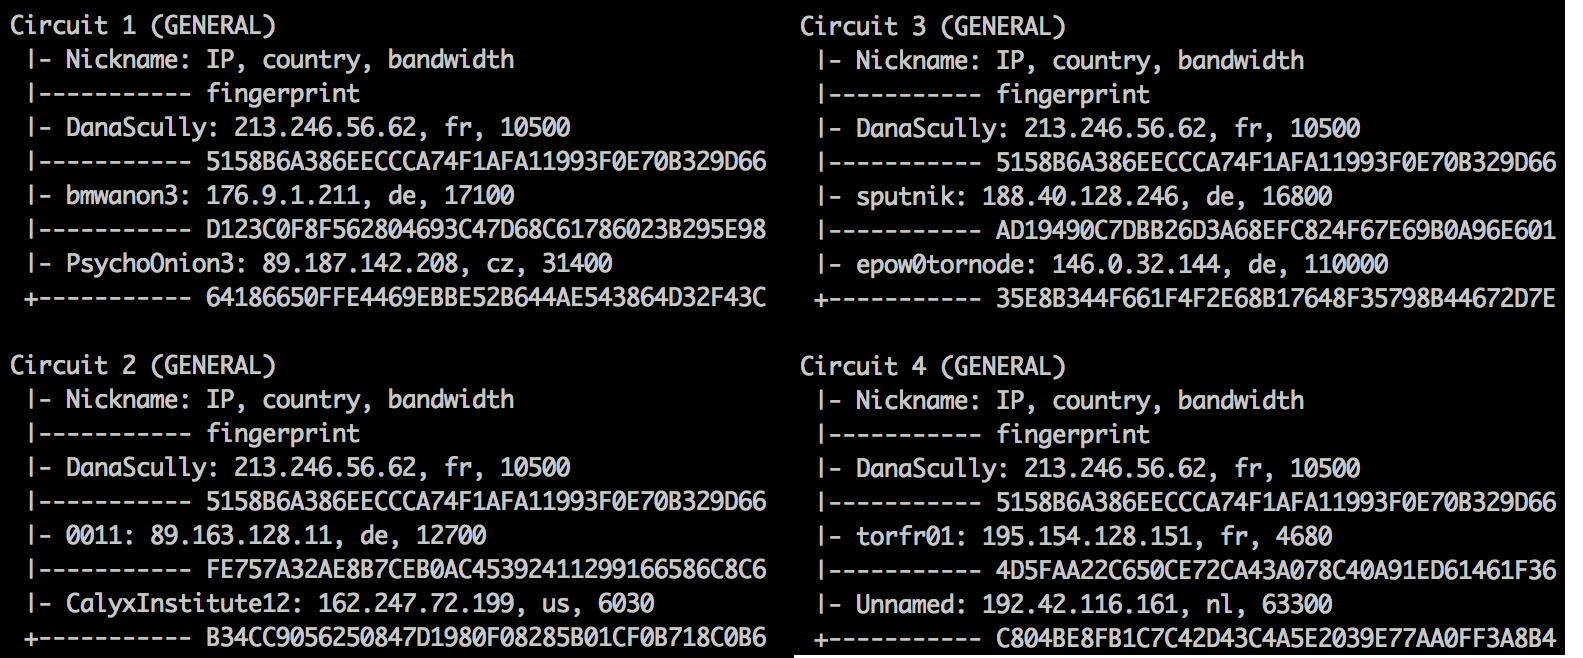
\includegraphics[scale=0.32]{circuits2.png}\\
 \caption{Current Circuits}
 \end{figure}
\end{answer}
\medskip

%
% Problem 1: Measuring latency
%
\newpage
 \subsubsection*{1.2 Measuring latencies}
1. Measures the difference between response times with or without going over Tor.\\
\medskip
\begin{answer}
Script available in {\bf shis\_hw4\slash measure\_latency.py}\\
It assumes that {\bf tor} is installed and already launched with {\bf SocksPort: 9150, ControlPort: 9151}\\
It assumes that {\bf PycURL} module is installed.\\
\medskip
Below is the list of supported argument, when running without arguments, the script call url provided in the assignment, and retry 10 times.\\
\medskip
Use ``-u" to set the url to connect\\
Use ``-r" to set number of retries\\
\end{answer}
\medskip

2. Give an estimate figure of how much overhead in latency Tor generates on a given connection. Run the above experiment 10 times, changing Tor identities (and thus, circuits) but connecting to the same website for each of the 10 runs, and provide a table summarizing the results.\\
\begin{answer}
\smallskip
%Data sample available in {\bf shis\_hw4\slash 1.2\_samples.txt}\\
Test URL: https://stem.torproject.org/tutorials/to\_russia\_with\_love.html\\
\smallskip
\begin{tabu} to 0.8\textwidth { | X[c] | X[c] | X[c] | X[c] | X[c] | X[c] | }
 \hline
  n & direct & tor & difference & abs diff & rank  \\
 \hline
 1 & 1.03 & 0.28 & 0.75 & 0.75 & 6  \\
  \hline
 2 & 0.92 & 0.18 & 0.75 & 0.75 & 6  \\
  \hline
 3 & 0.94 & 0.26 & 0.69 & 0.69 & 2.5 \\
  \hline
 4 & 0.95 & 0.26 & 0.69 & 0.69 & 2.5 \\
  \hline
 5 & 1.01 & 0.26 & 0.74 & 0.74 & 4  \\
  \hline
 6 & 0.94 & 0.18 & 0.75 & 0.75 & 6 \\
  \hline
 7 & 1.06 & 0.19 & 0.87 & 0.87 & 8 \\
  \hline
 8 & 0.90 & 0.27 & 0.63 & 0.63 & 1 \\
  \hline
 9 & 1.47 & 0.26 & 1.21 & 1.21 & 9 \\ 
  \hline
 10 & 1.46 & 0.18 & 1.28 & 1.28 & 10 \\
\hline
\end{tabu}\\
\bigskip
Using Wilcoxon Signed-Rank Test with the data above, we got test statistic value:\\
 \(T_-= 0\) \hspace{1em} \(T_+= | 1 + 2 + 3 + 4 + 5 + 6 + 7 + 8 + 9 | = 55\)\\
 \medskip
And we're trying to prove hypothesis \(H_1\) over \(H_0\):\\
\(H_0\): Distribution of response time of Tor(\(D_T\)) and direct connection(\(D_D\)) are identical\\
\(H_1\), \(D_T\) is the right shifted of the \(D_D\), i.e. most of Tor connection response time are longer than direct connection\\
 \medskip
Because we're testing \(D_T\) is the right shifted of the \(D_D\), so we will use test statistic \(T_-=0\)\\
Critical Values \(T_0 = 5\) in Wilcoxon Signed Rank one-tailed test when n=10, \(\alpha\) = 0.01 [1]\\
 \(T_- <= T_0\),  \(T_-\)  falls in the rejection region of \(T_0\)\\
So the data provide sufficient evidence to conclude that  \(D_T\) is the right shifted of  \(D_D\), at \(\alpha\) = 0.01.
i.e. The latency for Tor connection is higher than direct connection.\\
\end{answer}
\medskip

\newpage
3. Measure the latency of connecting to Tor hidden service. Compare it to the latency to its ``clearnet" version using the Tor network, and bypassing the Tor network. Explain why the hidden service address does not use https\\
\begin{answer}
%Data sample available in {\bf shis\_hw4\slash 1.2\_samples.txt}\\

%  DT 1111111
Compare between hidden service and clearnet version over Tor:\\
\smallskip
\begin{tabu} to 0.8\textwidth { | X[c] | X[c] | X[c] | X[c] | X[c] | X[c] | }
 \hline
  n & hidden & clear w/ Tor & difference & abs diff  & rank  \\
 \hline
 1 & 5.59 & 11.86 & -6.17 & 6.17 & -10  \\
  \hline
 2 & 1.68 & 1.43 & 0.25 & 0.25 & 4  \\
  \hline
 3 & 1.61 & 1.52 & 0.09 & 0.09 & 1 \\
  \hline
 4 & 1.81 & 1.29 & 0.52 & 0.52 & 6 \\
  \hline
 5 & 3.63 & 1.26 & 2.37 & 2.37 & 9  \\
  \hline
 6 & 0.74 & 1.27 & 0.75 & 0.75 & 8 \\
  \hline
 7 & 0.95 & 1.43 & -0.53 & 0.53 & -7 \\
  \hline
 8 & 0.76 & 1.27 & -0.51 & 0.51 & -5 \\
  \hline
 9 & 0.78 & 1.00 & -0.22 & 0.22 & -3 \\ 
  \hline
 10 & 0.75 & 0.87 & -0.12 & 0.12 & -2 \\
\hline
\end{tabu}\\
\bigskip
Using Wilcoxon Signed-Rank Test with the data above, we got test statistic value:\\
 \(T_-= | -10 + -7 + -5 + -3 + -2 | = 27,\) \hspace{0.5em} \(T_+= | 4 + 1 + 6 + 9 + 8 | = 28,\) \hspace{0.5em} \(T_0 = 5\) \\
 %Critical Values \(T_0 = 5\) in Wilcoxon Signed Rank one-tailed test when n=10, \(\alpha\) = 0.01 [1]\\
 Both \(T_+\) and   \(T_-\) is larger than critical value, thus fall out of \(H_0\)'s rejection region.\\
 \smallskip
 So there's no sufficient evidence to conclude that the distribution of latency of hidden service is different from the latency of the clearnet version over Tor.\\
 
 % DT 22222222222
\bigskip
 Compare between hidden service and clearnet version {\bf NOT} going through Tor:\\
\smallskip
\begin{tabu} to 0.8\textwidth { | X[c] | X[c] | X[c] | X[c] | X[c] | X[c] | }
 \hline
  n & hidden & clear w/o Tor & difference & abs diff  & rank  \\
 \hline
 1 & 5.59 & 0.15 & 5.44 & 5.44 & 10  \\
  \hline
 2 & 1.68 & 0.11 & 1.57 & 1.57 & 7  \\
  \hline
 3 & 1.61 & 0.11 & 1.50 & 1.50 & 6 \\
  \hline
 4 & 1.81 & 0.11 & 1.70 & 1.70 & 8 \\
  \hline
 5 & 3.63 & 0.10 & 3.53 & 3.53 & 9  \\
  \hline
 6 & 0.74 & 0.11 & 0.63 & 0.63 & 2 \\
  \hline
 7 & 0.95 & 0.10 & 0.85 & 0.85 & 5 \\
  \hline
 8 & 0.76 & 0.14 & 0.62 & 0.62 & 1 \\
  \hline
 9 & 0.78 & 0.11 & 0.67 & 0.67 & 4 \\ 
  \hline
 10 & 0.75 & 0.10 & 0.65 & 0.65 & 3 \\
\hline
\end{tabu}\\
\bigskip
 \(T_-= 0\) \hspace{1em} \(T_+= | 1 + 2 + 3 + 4 + 5 + 6 + 7 + 8 + 9 | = 55\)\\
 Critical Values \(T_0 = 5\) in Wilcoxon Signed Rank one-tailed test when n=10, \(\alpha\) = 0.01 [1]\\
 \(T_- <= T_0\),  \(T_-\)  falls in the rejection region of \(T_0\)\\
So the data provide sufficient evidence to conclude that  \(D_H\) is the right shifted of  \(D_C\), at \(\alpha\) = 0.01.
i.e. The latency for hidden service is higher than the clearnet version not going over Tor.\\
\smallskip
Connections with the Tor hidden services are going through Tor circuits, which are already all encrypted, so there's no need for https to reenforce confidentiality. Also the address of a hidden service came from the hash of the hidden service's public key, thus Tor client can verify the address using the public key got from the directory servers, there's no need for a CA in https model to sign a certification.

\end{answer}
\medskip

%
% Problem 1: Using exits to circumvent censorship
%
%\newpage
 \subsubsection*{1.3 Using exits to circumvent censorship}
1. Try to connect to http://dogo.ece.cmu.edu/tor-homework/public/ and http:// dogo.ece.cmu.edu/tor-homework/secret/ using a regular browser. How different are the results?\\
\begin{answer}
\medskip
When opening secret url with regular browser, it returns {\bf 403 Forbidden}.\\
When opening public url with regular browser, it shows ``{\bf the public part of the server is working}"


\end{answer}
\medskip

2. Write a Stem script to constrain Tor to specific exits in different countries.\\
\begin{answer}
\medskip
Script available in {\bf shis\_hw4\slash exit\_node.py}\\
It assumes that {\bf tor} is installed and added to PATH, and the {\bf PycURL} module is installed.\\
It assumes port {\bf 9150, 9151} are not occupied, and will launch with {\bf SocksPort: 9150, ControlPort: 9151} \\
\medskip
Below is the list of supported argument, when running without arguments, the script call url provided in the assignment, and try to switch circuits 5 times in a country.\\
\medskip
Use ``-u" to set the url to connect\\
Use ``-r" to set number of s to switch circuit for exist nodes in a country\\
\end{answer}
\medskip

3. Use your script to find as many countries as possible in which the website http://dogo.ece. cmu.edu/tor-homework/secret/ is not blocked. Provide a list of these countries, as well as the exact date/time at which you made each request verifying that each of these countries was not blocked.\\
\begin{answer}
Find GB returns 200, 2015-12-02 03:16:32\\
Find RU returns 200, 2015-12-02 03:16:35\\
Find FR returns 200, 2015-12-02 03:17:19\\
Find AU returns 200, 2015-12-02 03:17:24\\
Find PL returns 200, 2015-12-02 03:17:28\\
Find CH returns 200, 2015-12-02 03:19:51\\
Find HU returns 200, 2015-12-02 03:34:21\\
Find GR returns 200, 2015-12-02 03:36:40\\
Find LU returns 200, 2015-12-02 03:47:58\\
Find RO returns 200, 2015-12-02 11:04:33\\
Find SE returns 200, 2015-12-02 11:14:24\\
\end{answer}
\medskip



%
% Problem 2: 
%
\newpage
\begin{center}
\textbf{Problem \#2 : WikiLeaks and anonymity}
\end{center}

1. Decide whether you support banning the design and use of anonymous networks or not, and prepare four arguments to support your position, and one mitigating factor \\
\begin{answer}
I oppose banning anonymous networks.

\end{answer}
\bigskip

[1] Stat.ufl.edu,. (2015). Retrieved 4 Dec. 2015, from http://www.stat.ufl.edu/~winner/tables/wilcox\_signrank.pdf


\end{document}